\documentclass[runningheads,a4paper]{llncs}

\usepackage{amssymb}
\usepackage{graphicx}
\usepackage{url}
\usepackage{color}
\usepackage{CJK}
\usepackage{url}
\usepackage[ruled]{algorithm2e}
\usepackage{amsmath}
\usepackage{graphicx}
\usepackage{enumerate}
\usepackage{multirow}

\urldef{\mailthu}\path|{lmy13}@tsinghua.edu.cn|
\urldef{\mailsy}\path|{fantasysy}@sina.com|
\newcommand{\keywords}[1]{\par\addvspace\baselineskip\noindent\keywordname\enspace\ignorespaces#1}
\newcommand{\para}[1]{\vspace{0.1cm}\noindent\textbf{#1}}

\begin{document}
\begin{CJK*}{UTF8}{song}
\mainmatter

\title{Building Large-Scale Cross-lingual Knowledge Base from Multi-Encyclopedia}
\titlerunning{Bilingual Knowledge Base}
\author{Mingyang Li$^\dag$ \and Yao Shi$^\dag$ \and Zhigang Wang$^\dag$}
\authorrunning{Mingyang Li et.al}

\institute{$^\dag$Tsinghua National Laboratory for Information Science and Technology,\\
Department of Computer Science and Technology,\\
Tsinghua University, Beijing 100084, China\\
\mailthu\\
\mailsy\\
}

\maketitle

\begin{abstract}

Cross-lingual Knowledge Bases are important for global knowledge sharing. However, there are few Chinese-English knowledge bases due to the following reasons: 1) the scarcity of Chinese knowledge; 2) the number of current cross-lingual language links is limited; 3) the incorrect relation in semantic taxonomy. In this paper, a large-scale cross-lingual knowledge base(CLKB) is build to solve the above problems. The CLKB is based on English and Chinese Wikipedia as well as Baidu Baike and Hudong Baike. An extension method is used to increase language links while a pruning approach is used to refine taxonomy. Totally, there are XXX classes, XXX instances, XXX properties referred in the CLKB. Moreover, the paper provides visualization webpages of knowledge and a SPARQL endpoint accessing to the established CLKB.

\keywords{Knowledge Base, Semantic Web, Ontology, Cross-lingual}
\end{abstract}

\section{Introduction}

As the Web is evolving to a highly globalized information space, sharing knowledge across different languages is attracting increasing attentions. Multilingual knowledge bases have significant applications such as multi-lingual information retrieval, machine translation and deep question answering. DBpedia, by extracting structured information from Wikipedia\footnote{{\tt http://www.wikipedia.org/}} in XXX different languages, is a multi-lingual multi-domain knowledge base and becomes the nucleus of LOD\footnote{{\tt http://linkeddata.org/}}. Obtained from the automatic integration of WordNet\footnote{{\tt http://wordnet.princeton.edu/}} and Wikipedia, YAGO, MENTA and BabelNet are other famous large multi-lingual knowledge bases.

However, most non-English knowledge in those knowledge bases is pretty scarce. Figure \ref{fig_stat} shows a simplified long tail distribution of the number of articles on six major Wikipedia language versions. Due to the imbalance of different Wikipedia language versions, the knowledge distribution across different languages is highly unbalanced in those knowledge bases which are generated from Wikipedia. For instance, DBpedia contains XXX English instances but only XXX Chinese instances. On the other hand, the Chinese Hudong Baike\footnote{{\tt http://www.baike.com/}} and Baidu Baike\footnote{{\tt http://baike.baidu.com/}}, both containing more than 6 million articles, are even larger than the English Wikipedia. If a knowledge base could be established between English Wikipedia and Chinese Hudong Baike, an English-Chinese knowledge base with much higher coverage in Chinese can be constructed.
\begin{figure}[h]
\centering
  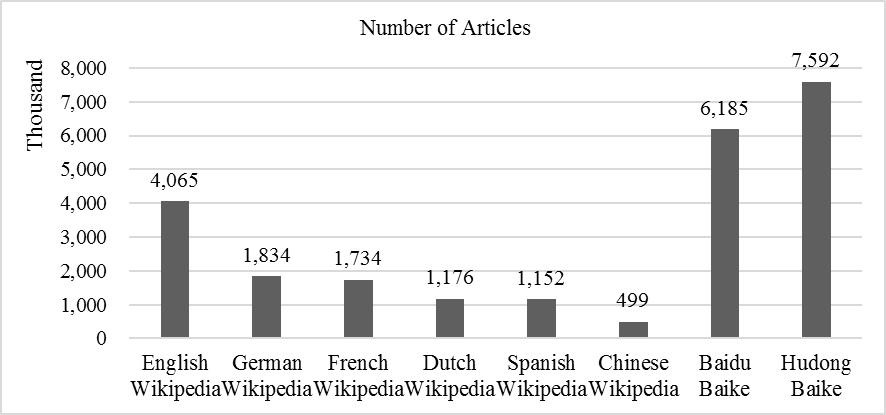
\includegraphics[width=11cm]{fig_stat.png}\\
  \caption{Number of Articles on Major Wikipedias, Baidu Baike and Hudong Baike}
  \label{fig_stat}
\end{figure}

To enrich the Chinese knowledge, we try to build a large-scale English-Chinese knowledge base by semantifying four heterogeneous online wikis, which are English Wikipedia, Chinese Wikipedia, Hudong Baike and Baidu Baike. In this paper, we propose a unified framework to build such a knowledge base. The framework contains XXX steps: XXX, XXX, and XXXX. The generated knowledge base contains XXX classes, XXX instances and XXX properties. An online system supporting keyword search and SPARQL endpoint is also developed.

This non-trivial task poses the challenges as follows.
\begin{enumerate}
  \item The cross-lingual links are highly limited inside Wikipedia. For instance, there are only XXX English-Chinese links in Wikipedia. How could we find enough English-Chinese \verb"owl:sameAs" relations?
  \item The subsumption relations of the online wikis' category systems contain lots of noise. For example, in English Wikipedia ``Wikipedia-books-on-people", which is actually \verb"subClassOf" ``Books", is taken as the sub-category of ``People" mistakenly. How could we detect those incorrect semantic relations?
\end{enumerate}

Driven by these challenges, we propose a unified framework to build a English-Chinese knowledge base from four heterogeneous online wikis. Specifically, our work makes the following contributions.
\begin{enumerate}
  \item We extend the cross-lingual link set by employing a cross-lingual knowledge linking discovery approach for class and instance, and analyzing templates in Wikipedia for property.
  \item We prune the original taxonomy, which is extracted from encyclopedia category system, to retrieve more precise \textit{subClassOf} and \textit{instanceOf} relations in ontology.
  \item Both website and SPARQL endpoint are provided for public query operations over our knowledge base.
\end{enumerate}

The rest of the paper is organized as follows. Section \ref{sec:pd} presents some basic concepts and the problem formulation. In Section \ref{sec:dp} we presents we present our detailed approaches. The experimental results are reported in Section \ref{sec:result}. Some related work are described in Section \ref{sec:work}. Finally we conclude our work in Section \ref{sec:con}.

\section{Problem Definition}
\label{sec:pd}
In this section, we firstly introduce the encyclopedias used to build and enrich our knowledge base. Then we give definitions about ontology and knowledge base. At last we describe our task in this work.

\subsection{Encyclopedias}
\label{sec:encyclopedias}
\subsubsection{Wikipedia}
Nowadays, Wikipedia is the largest data store of human knowledge. It was launched in 2001 and has hold over 35 million articles in 288 languages by 2015. Out of these, English articles contribute most. The imbalance of different language articles makes ontologies based on Wikipedia-only behave badly in cross-lingual. Thus, more Chinese encyclopedias are necessary to enrich Chinese source.

Among the large-scale monolingual Chinese encyclopedias currently, Baidu Baike and Hudong Baike are the most content-rich. Hudong Baike was founded in 2005 and contains more than 12 million articles with about 9 million experts' contribution until 2015. Meanwhile, Baidu Baike maintains more than 11 million articles.

Here, we consider an encyclopedia wiki as a collection of articles, category system, which can be defined as: $W = <A,C>$, where A denotes articles, C denotes categories in W.

\subsection{Wiki Pages}
Articles from the four sources are similar in structure. Usually they provide two important elements with potential semantic information, category system and articles. A category system represents the relations between categories as a tree by the relation \textit{subCategoryOf}. Fig.\ref{fig:hudong-taxonomy} shows a screenshot of Hudong Taxonomy. An article describes an entity with rich information created and modified by several verified editors. Besides, each article is linked to one or more categories by \textit{articleOf} relation. In general, there are five elements can be exploited in each article page:
\begin{figure}
    \centering
    \begin{minipage}[t]{0.8\textwidth}
        \centerline{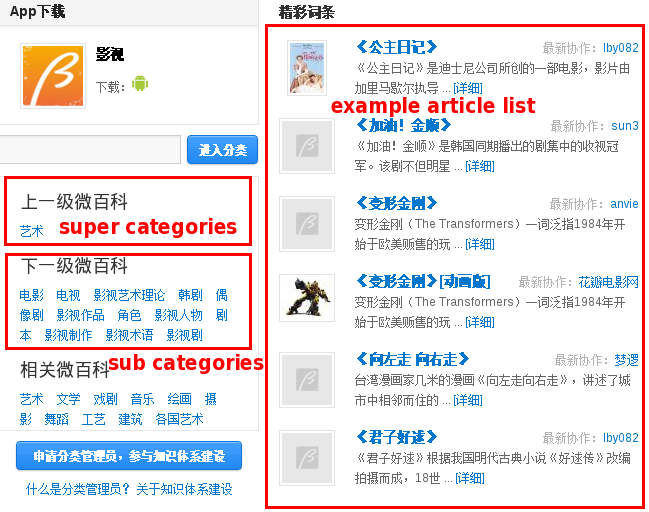
\includegraphics[width=0.8\columnwidth]{fig/hudong-taxonomy2}}
        \caption{Taxonomy in Hudong}
        \label{fig:hudong-taxonomy}
    \end{minipage}%
\end{figure}
\begin{itemize}
  \item Title: A Title is the label of an entity, which is unique so that it can be used to distinguish entities.
  \item Abstract: An abstract is a brief summary of the entity. It's always the first paragraph of an article.
  \item Infobox: Most of articles contain infobox. An infobox maintains structured data which are subject-attribute-value triples formalized as a table. Information in this table includes important properties of an entity.
  \item Links: Links are entries to other articles within the encyclopedia. They lead readers to reference articles. Actually, they represent the relations between the current article and other articles.
  \item Category: The categories that an article belongs to are usually listed at the bottom of article page, shown as tags. An article has \textit{articleOf} relation with its categories.
  \item URL: Each article has an HTTP url to identify itself on web.
\end{itemize}

Fig. \ref{fig:interstellar} shows a snap of an article in Chinese Wikipedia.
\begin{figure}[ht]
    \centerline{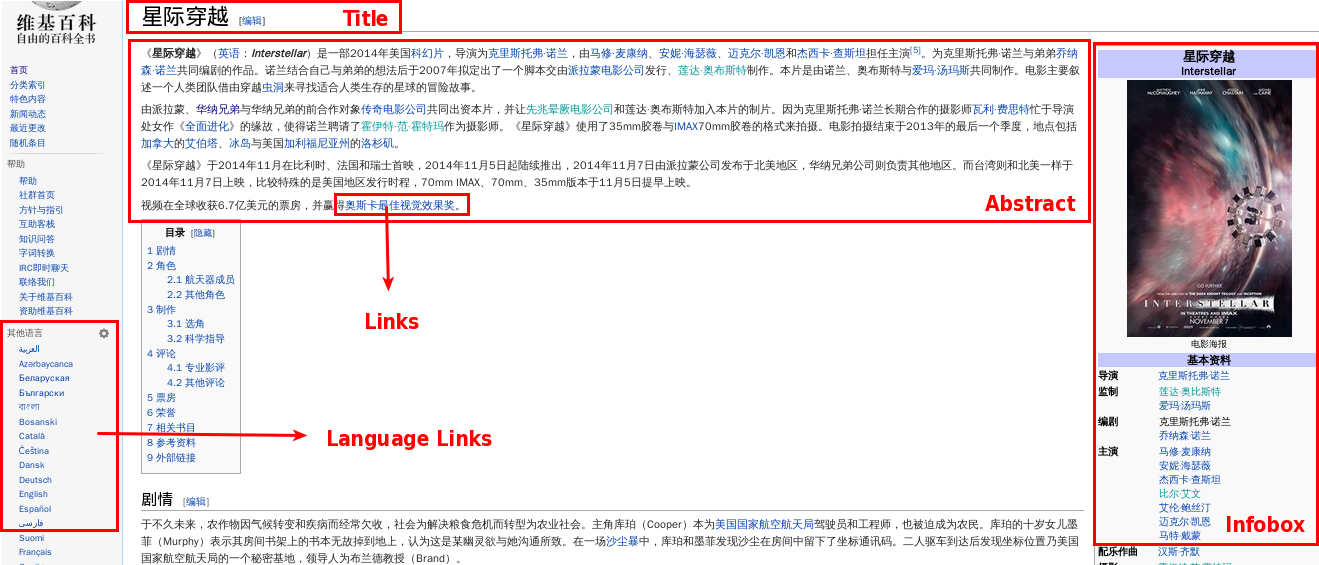
\includegraphics[width=1\columnwidth]{fig/interstellar}}
    \caption{A snap of Interstellar(Film) article in Chinese Wikipedia}
    \label{fig:interstellar}
\end{figure}%

The elements of each article $a$ can be defined as follow:
\begin{equation}
    a = <Ti(a),Ab(a),Li(a),In(a),C(a),U(a)>
\end{equation}
where $Ti(a),Ab(a),Li(a),In(a),C(a),U(a)$ denotes title, abstract, links, infobox, category tags, url of article $a$.

Notably, articles in Wikipedia follow templates specified by Wikipedia when being edited. A template defines items that a group of article should fill. Besides, infoboxes are also generated based on certain templates recommended by Wikipedia. For example, The infobox in film 星际穿越(Interstellar) is edited according to the Template \emph{Infobox film}, which maintains a property set of films. An Infobox $In(a)$ contains a set of attribute-value pairs {$p_{1}$, $p_{2}$,...}. We denote infobox template as $T(a)$. Templates specify certain attributes, which are usually different from those displayed on the webpage. Thus, we define an attribute-value pair as a triple $p=<tl,dl,v>$, where $tl$ is attribute label in template, $dl$ is displayed label in web page and $v$ is the corresponding value. The value maybe a text or a reference to another entity.

Moreover, in Wikipedia, some article pages have language links which help readers switch to other language-version within the same article. Fig. \ref{fig:interstellar}shows language links of \emph{Interstellar} on the right column of the Wikipedia page. As to an article $a$ containing multi-language content in Wikipedia, $L_{e}$ and $L_{z}$ denotes its article links, usually titles, in English and Chinese separately. Thus, to a $cl$ in $CL$, $cl(a) = <L_{e}(a), L_{z}(a)>$.

\subsection{Ontology and Knowledge Base}

An ontology is a formal specification of a group of entities. In our work, an ontology is described as a 4-tuple:
\begin{equation}
    O = <C,I,P,H^C>
\end{equation}
where $C$, $I$, $P$ are the sets of classes, instances, and properties, respectively. $H^C$ represents the hierarchical relationships of classes. A Taxonomy includes two types of relationships, which are \textit{subClassOf} of class-class and \textit{instanceOf} of class-instance.

A cross-lingual knowledge base is a database conform to a cross-lingual ontology. Taking advantage of language links in $CL$, several monolingual-ontologies generated from various sources can be merge into one cross-lingual ontology.  Thus a knowledge base can be defined as:
\begin{equation}
    KB = <O_{i}, CL>
\end{equation}
where $O_{i}$ denotes the ith monolingual-ontology, $CL$ represents the cross-lingual link set.

\subsection{Cross-lingual Knowledge Base Building}

In this paper, our task is to build an Cross-lingual Knowledge Base(CLKB) assembling knowledge from several English or Chinese encyclopedia sources. Given four encyclopedia datasets $W_{1},W_{2},W_{3},W_{4}$, we get $O_{i}$ including class list $C_{i}$, instance list $I_{i}$, property list $P_{i}$, taxonomy $H^C_{i}$ of each dataset $W_{i}$ by extracting. We then enrich the extracted language-link set $CL$ using an link-discovery extension method. We also refining taxonomy by checking if an \textit{articleOf} or \textit{subCategoryOf} is really an \textit{instanceOf} or \textit{subClassOf} relationship. Our final output is an English-Chinese ontology  with SPARQL endpoint though process of combine $O_{i}$ by utilizing language links in $CL$.

The whole building procedure is shown in Fig. \ref{fig:procedure}
\begin{figure}[ht]
    \centerline{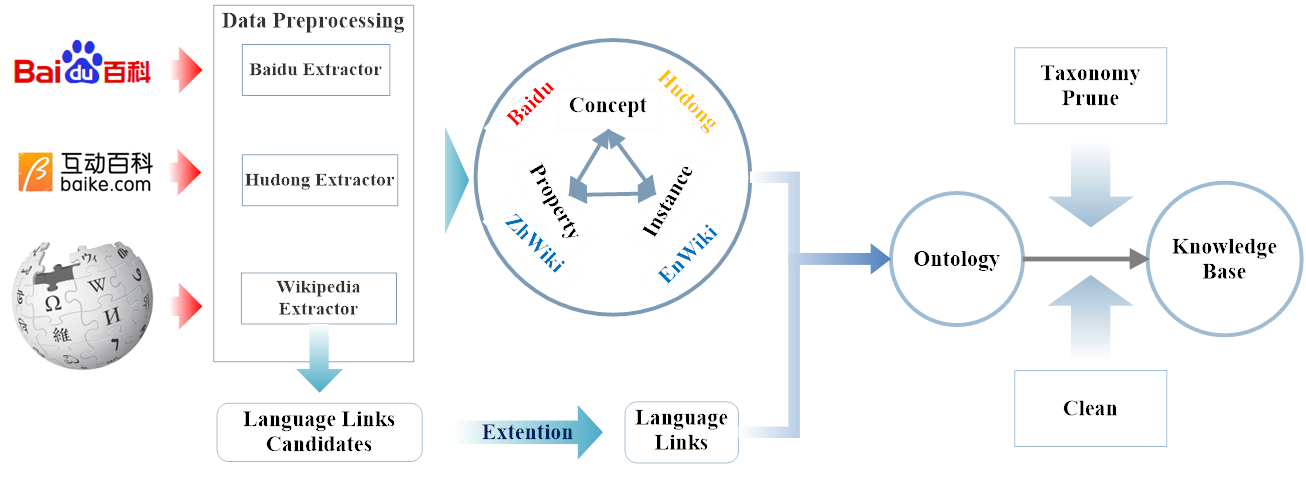
\includegraphics[width=1\columnwidth]{fig/procedure}}
    \caption{Procedure of building our cross-lingual knowledge base}
    \label{fig:procedure}
\end{figure}%
We extract information from four sources, Baidu Baike, Hudong Baike, Chinese Wikipedia and English Wikipedia. Considering the different data format of each source, that is, html code page of Baidu and Hudong with different layout, and XML format of Wikipedia dump file, various extractors should be employed. After data parsing, we get four ontologies each source. Going through the process of taxonomy pruning, we delete some incorrect relations. At last Using the extended language links, we combine the four ontologies into a cross-lingual knowledge base.

\section{Semantic Data Extraction}
\label{sec:dp}
Semantic data extraction aims to achieve a structured dataset from the input encyclopedias, preparing for the knowledge base construction. Specifically, we extracts classes from category taxonomy, instances according to articles, and properties based on infoboxes and its templates.

\subsection{Class Extraction}
\label{sec:ce}
A class is defined as a type of similar instances. For example, the class of instance \emph{Interstellar} is \emph{Movie}. In general, a class has super classes and sub classes. Classes comprise a taxonomy which presents a backbone of an ontology. In an encyclopedia, a category groups several articles and also has super-categories and sub-categories. Therefore we can extract classes based on existing category system.

However, the whole taxonomy can not directly transform from category system because of the following problems:
\begin{itemize}
    \item There are auxiliary categories in Wikipedia, which help arrange specific articles or category pages. For example, \emph{Lists of artists} or \emph{Food templates}.
    %s\item Some sub-category links in the category system maybe inconsistent. Some categories may contain itself as sub-category, or contain sub-category that also be the super-category of it. As Fig. \ref{fig:category-mistakes} shows: In Hudong, the sub-category of 国家元首(Head of State) contains itself as a child, which causes a circle in taxonomy tree. Meanwhile, in Wikipedia, \textcolor{red}{例子}
    \item Some categories relate to only one or two articles. According to the definition of class, such categories are less representative to a group of instances, therefore it's unwise to retain it as class.
\end{itemize}

   To obtain a more precise $H^C$ in a $W$, we remove such categories in all encyclopedias, then build the original class hierarchy $H^C$ using the remaining categories.

However, among the relations there are still incorrect samples. For example, \emph{Tsinghua University} is not an entity of \emph{Haidian District}, but relates to. Thus we will prune the taxonomy later.

\subsection{Property Extraction}
\label{sec:pe}
A property is defined as an attribute of an entity. It represents the relation between two instances or an instance and its value. We divided properties into two types: object property, whose value is an individual, such as \emph{directed by}; datatype property, whose value is a literal text, such as \emph{birth date}. Considering both content and infobox of an article, we extract two kinds of properties, general-properties and Infobox-properties.

\subsubsection{General-properties}
Characteristics of an entity are regarded as general-properties, including label, abstract, and url. General-properties describe general information of an entity. We define three datatype properties as general-properties for a given article $a$: (1) label property; (2) abstract property; (3) URL property.

\subsubsection{Infobox-properties}
Attributes acquired from infobox are considered as Infobox-properties, such as 上映时间(release date), 导演(directed by) in a movie's infobox. The type of a property, datatype or object, depends on the type of the value. Ordinarily, a plain text value marks the property as datatype while an entity reference determines the property as objecttype. For example, the attribute 上映时间(release date) can be defined as a datatype property as its value is a datetime string. Meanwhile, 导演(directed by) can be an object property because its value points to a person who directed the movie.

We are challenged when extracting properties from infoboxes:
\begin{itemize}
    \item In Wikipedia, the attribute label displayed in the webpage infobox is inconsistent with it in the published dump file. Fig.\ref{fig:infobox-template} gives a mapping result of display labels and dump labels in \emph{Interstellar}' infobox. The left is infobox, the middle is a snap from dump file in Wikipedia. As we've seen, attribute label in infobox is different from it in dump file. We explore the display labels as property labels in Wikipedia rather than dump labels extracted from raw data.
    \begin{figure}[ht]
        \centerline{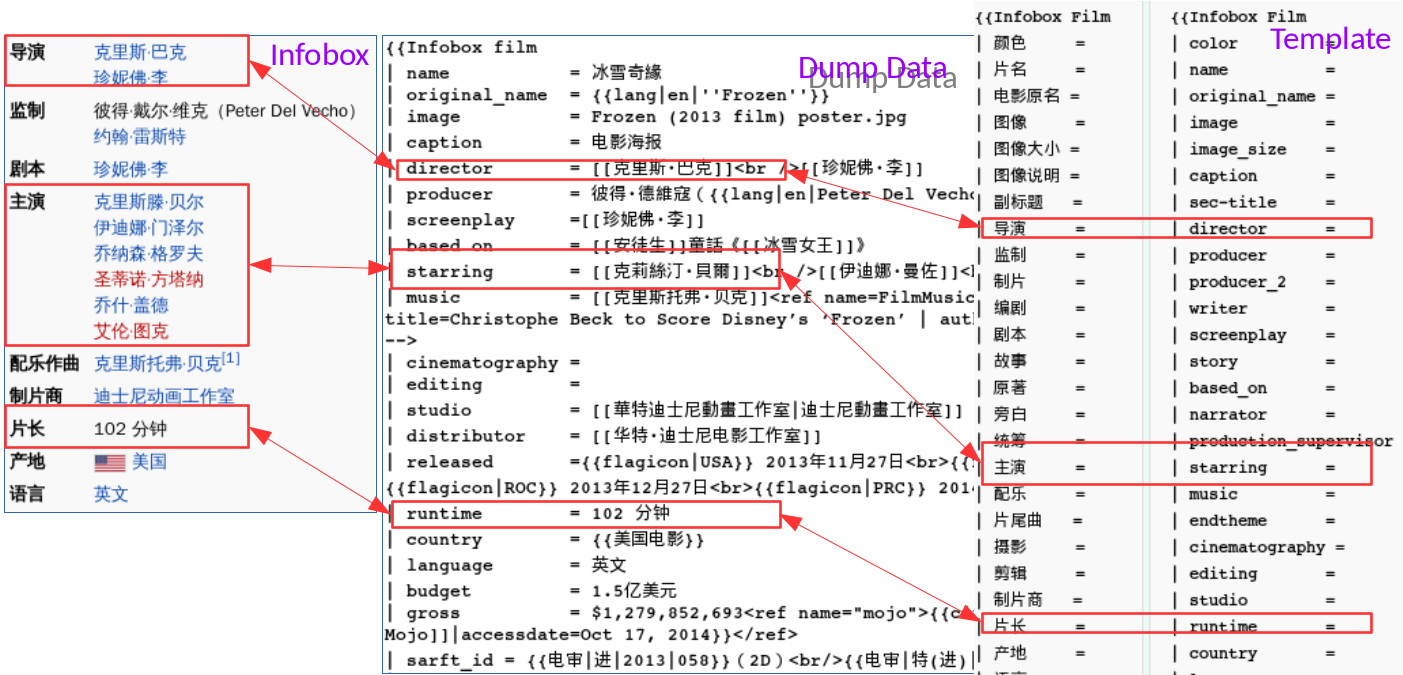
\includegraphics[width=1\columnwidth]{fig/infobox-template}}
        \caption{Comparison of display label and dump label in \emph{Interstellar} infobox}
        \label{fig:infobox-template}
    \end{figure}%
\item There are special characters in labels. Wikipedia usually uses hyphen "-" or dot "•" to mark sublabels. For example, \emph{population} property has sub-properties "-Density" and "-Urban". In addition, odd signs, such as colon or asterisk, may occur in Baidu or Hudong property labels by mistake.
\end{itemize}

To solve the problems above, we take advantage of template information. Specifically, Wikipedia institutes rules of rendering label in templates. For example, movie infobox follows template \emph{Infobox film}, which is shown on the right of Fig.\ref{fig:infobox-template}, where both display labels and dump labels come from. When a dump label occurs in dump file, we replace it by its mapping display label.

\subsection{Instance Extraction}
\label{sec:ie}
In encyclopedia, an article describes unique entity in the world. Therefore we can extract an article as an instance. During the extraction, illustrative or structure-related articles in Wikipedia are deleted, including category list pages and template documentations.

We harvest four types of information during this stage. (1) General-properties of instance, including title as label property value, first paragraph as abstract property value and HTTP URL as URL property value. (2) Infobox-properties which are acquired via extracting from the infobox in the article; (3) $articleOf$ relation with categories listed at the bottom of article page. For example, 美国科幻片(American science fiction films) is a category of Interstellar; (4) Reference relation with other instances according to links in the content. We gain the reference $Li(a)$ between the current instance and others, such as 华纳兄弟(Warner Bros.).

\section{Cross-lingual Integration}
\label{sec:clkbb}

To construct a cross-lingual knowledge base with existing structured data, firstly we gather cross-lingual links which can help match the same entity in two languages and extend the link set. Secondly, we integrate this four encyclopedias, which is to say, respectively merging concepts, instances and properties from the four sources if they represent the same thing. Thirdly, we prune the taxonomy generated from concept relationships to make it more accurate. At last, we make instances and properties attached to complete the cross-lingual knowledge base construction.

\subsection{Cross-lingual Linking}
There are \textcolor{red}{number} cross-lingual links between English and Chinese, which constitute the initial cross-lingual link set of concepts and instances. Moreover, we utilize the language-independent method in \cite{wang2012cross} to extend the language-link set. With the linkage factor graph model, we harvest a cross-lingual links extension as many as 20 thousands with an ideal precision 85.5\% and a recall of 88.1\% between English Wikipedia and Baidu Baike.

However, due to using templates, Infobox-properties have no obvious cross-lingual links. To acquire such links, we take the following steps: (1) Given a matched template, which means $T_{e}$ and $T_{z}$ are cross-lingual pairs, find the display labels mapping the same dump label. That is to say, to two pairs, $p_{e}$ in $T_{e}$ and $p_{z}$ in $T_{z}$, if $tl_{e}$ is equal to $tl_{z}$, $<dl_{e},dl_{z}>$ are cross-lingual properties; (2) Given the English and Chinese infoboxes of a matched instance, compare their templates, which are English template $T_{e}(a_{e})$ and a Chinese template $T_{z}(a_{z})$ in which $a_{e}$ and $a_{z}$ direct to the same entity, find the matched display labels mapping to the same dump label; (3) Given the English and Chinese infoboxes of a matched instance, for datatype properties, compare the similarity of literal value; to object properties, check whether the value refer to the same entity.

However, due to using templates, Infobox-properties have no obvious cross-lingual links. To acquire such links, we take the following steps:
\begin{enumerate}[1)]
    \item Given two matched templates, $T_{e}$ and $T_{z}$, find the display labels mapping the same dump label. That is to say, to $p_{e}$ in $T_{e}$ and $p_{z}$ in $T_{z}$, if $tl_{e}$ is equal to $tl_{z}$, $<dl_{e},dl_{z}>$ are cross-lingual properties;
    \item Given the English and Chinese infoboxes of two matched articles $a_{e}$ and $a_{z}$ direct to the same entity, compare their templates, English template $T_{e}(a_{e})$ and Chinese template $T_{z}(a_{z})$, find the matched display labels mapping to the same dump label; 
    \item Given the English and Chinese infoboxes of a matched instance, for datatype properties, compare the similarity of literal value; for object properties, check whether the value refer to the same entity.
\end{enumerate}

In order to make all encyclopedias link to each other, we unify the same class, instance and property from four sources, and give them unique identifiers. For instance, we merge instances by the following steps: (1) Merge all instances extracted from Chinese encyclopedias by instance title. (2) To a $L_{z}$, find whether there is an English cross-lingual link $L_{e}$ in $CL<L_{e}, L_{z}>$. If exists, make the two as one instance and identify it using an ID, else number it with a new ID.

The process of unifying class and property is the same as instance. Meanwhile, all the relations in all sources are kept to prevent loss of information.

\subsection{Taxonomy Prune}
\label{sec:tp}

As a result of combining multi-source information without verifying, there is noise in taxonomy. For example, \textcolor{red}{example}. Therefore, we introduce the method from\cite{wang2014cross} to detect the correct \textit{subClassOf} and \textit{instanceOf} relations from \textit{subCategoryOf} and \textit{articleOf}. Table. \ref{tab:} shows some examples of correct relations. In particular, some language-dependent literal and language-independent structural features are defined to vectorize each class or instance. Employing these features, a Yes-or-No binary-classification model is trained based on Logistic Regression. The whole process is iterative by retraining model with assured result to get higher precision. The prediction results are validated by cross-lingual information.

The ideal result after pruning is a tree, whose edges, nodes, and leaves separately denote relations, classes and instances. However, since getting rid of incorrect entity relations without consideration of integrity, a forest result is inevitable.

\section{Result}
\label{sec:result}

\subsection{Extracted Knowledge Base}
We collect the resources from 4 wiki sites, English and Chinese Wikipedia dump files in Dec, 2014, Hudong html pages until May, 2014, and Baidu html pages until September, 2014. Each of the wikis has three types of information, which can be utilized for constructing our ontology, namely, specific articles, classification system, and attribute of articles. We extract each raw data, then form the extracted information into well-structured data. Table \ref{tab:extract-result} the result we get after elementary extraction on 4 different wiki sources.

\begin{table}[h]
\small
\centering
\caption{Statistics of elementary extraction result}
\label{tab:extract-result}
    \begin{tabular}{|l|l|l|l|l|}
        \hline
                 & Enwiki  & Zhwiki & Hudong  & Baidu   \\ \hline
        \#Instance & 4304113 & 662650 & 5590751 & 5622404 \\ \hline
        \#Class    & 982432  & 159705 & 31802   & 1300    \\ \hline
        \#Property & 43976   & 18842  & 1187    & 139634  \\ \hline
    \end{tabular}
\end{table}

Besides, we obtain 227 thousand language links between English and Chinese in Wikipeidia, and increase the number by 191 thousand enwiki-baidu language links.

We create URIs to identify each element and provide corresponding information if users look up elements over HTTP protocol to achieve the knowledge base. Table \ref{tab:uris} lists the defined URIs.
\begin{table}[h]
\small
\centering
\caption{URIs for class, instance, property in our knowledge base}
\label{tab:uris}
    \begin{tabular}{|c|c|}
        \hline
        Type     & URI                     \\ \hline
        Class    & http://clkb/class/id  \\ \hline
        Instance & http://clkb/instance/id \\ \hline
        Property & http://clkb/property/id \\ \hline
    \end{tabular}
\end{table}

After fusing the heterogeneous resources, we harvest a cross-lingual graph with 1,093,855 classes, 200,223 properties, and 11,721,238 instances respectively. With different methods of extraction and language link discovery, these three kinds of entries show different results in languages. We give a breakdown of both Chinese knowledge and English knowledge in Table \ref{tab:kb-result}.

\begin{table}[h]
\small
\centering
\caption{Statistics of our knowledge base}
\label{tab:kb-result}
\begin{tabular}{|l|l|l|l|l|l|l|}
\hline
\multicolumn{1}{|c|}{} & \multicolumn{2}{c|}{Classes}      & \multicolumn{2}{c|}{Instance}                   & \multicolumn{2}{c|}{Property}    \\ \hline
English                & 982,982   & 89.86\%                & 4,311,719              & 37.79\%                & 54,802  & 27.37\%                \\ \hline
Chinese                & 176,648   & 16.15\%                & 7,842,117              & 66.9\%                 & 167,083 & 83.45\%                \\ \hline
Cross-lingual          & 65,775    & 6.01\%                 & 432,598                & 3.7\%                  & 21,662  & 10.82\%                \\ \hline
Only English           & 917,207   & 83.9\%                 & \multicolumn{1}{c|}{-} & \multicolumn{1}{c|}{-} & 33140   & 16.6\%                 \\ \hline
Only Chinese           & 110,873   & 10.1\%                 & \multicolumn{1}{c|}{-} & \multicolumn{1}{c|}{-} & 145,421 & 72.6\%                 \\ \hline
Sum                    & 1,093,855 & \multicolumn{1}{c|}{-} & 11,721,238             & \multicolumn{1}{c|}{-} & 200,223 & \multicolumn{1}{c|}{-} \\ \hline
\end{tabular}
\end{table}

Our knowledge graph is organized in Openlink Virtuoso, which is a data management platform rendering various services, including triple store.

\subsection{Web Access to Knowledge Base}
We provide a website to present an intuitive graph of our knowledge in the forms of class, instance and property. Fig.\ref{fig:xlore} shows sample pages of the integrated data. Users can choose language preference which is convenient for both English speaker and Chinese speaker. In the class webpage, we exhibit the label, super classes, subclasses, related topics, properties and instances of the specific class in bilingual way on condition that the corresponding English entries or Chinese entries exist.  In the instance webpage we display bilingual label, super classes, related classes, abstract, property key value pairs, images and references. In the property webpage, we present bilingual label, domains, ranges, and related instances of each property.
\begin{figure}[ht]
    \centerline{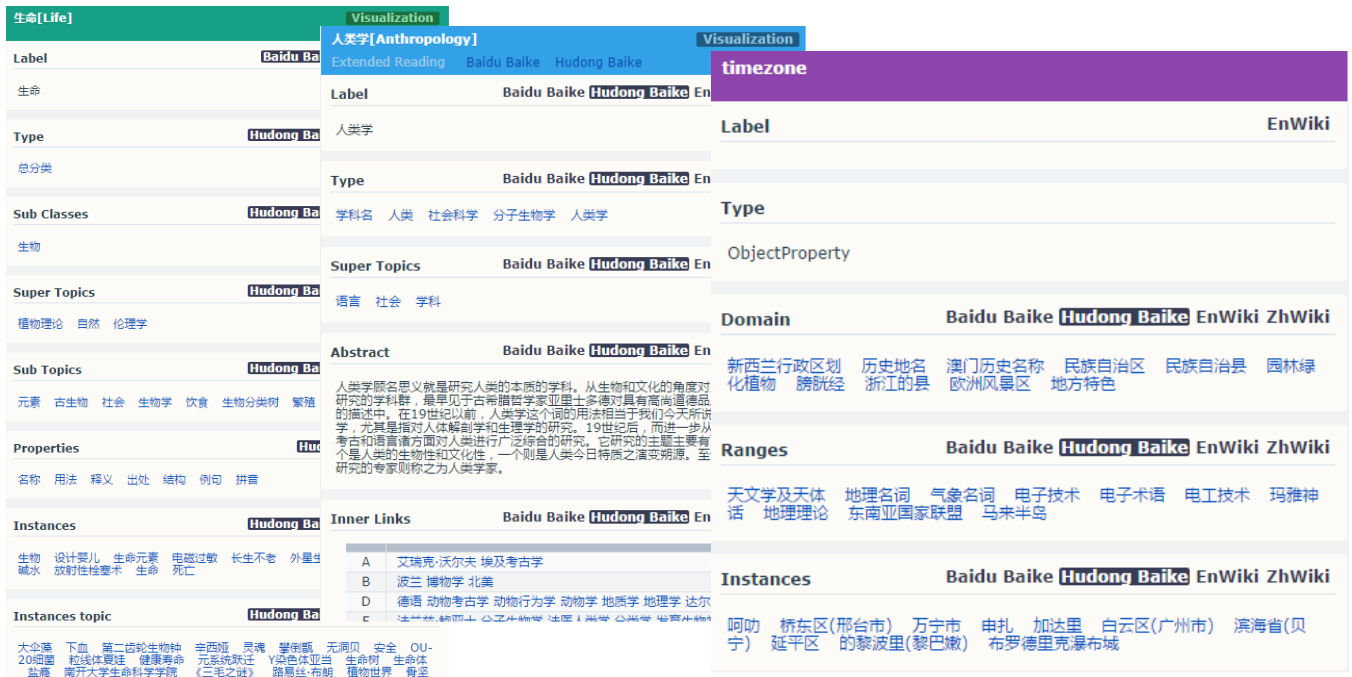
\includegraphics[width=1\columnwidth]{fig/xlore}}
    \caption{Sample Pages of Class, Instance and Property}
    \label{fig:xlore}
\end{figure}%
Beside these user-friendly pages, we provide two ways to access our knowledge base: via the search engine shown in Fig.\ref{fig:search-engine}, or via SPARQL endpoint shown in Fig.\ref{fig:sparql-endpoint}. For general users, they can make a query by inputing related text into searchbox and search to get entities with similar label. To present practicable result, An index is generated over all entities. We as well provide SPARQL interface for professional users to query our knowledge graph. Users can choose the language tags of their desired results by \textbf{"filter(langMatches(?label),"en"))"} or \textbf{"filter(langMatches (?label),"zh"))"}. For example, to get the English label of an instance, the query is: select * where {$<$\url{http://clkb/instance/100}$>$ $<$\url{http://www.w3.org/2000/01/rdf-schema#label}$>$ ?label. filter(langMatches(?label),"en"))}.

%\begin{figure}
%    \centering
%    \begin{minipage}[t]{0.8\textwidth}
%        \centerline{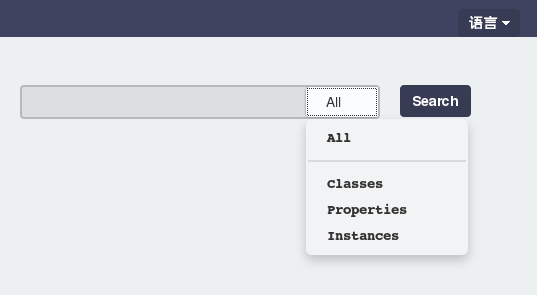
\includegraphics[width=0.8\columnwidth]{fig/search-engine}}
%        \caption{A Sample Query for Using Search Box }
%        \label{fig:search-engine}
%    \end{minipage}%
%    \begin{minipage}[t]{0.8\textwidth}
%        \centerline{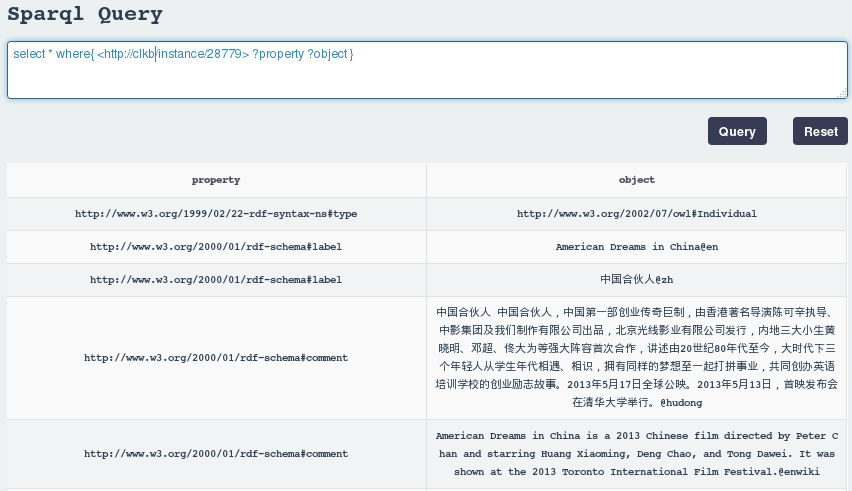
\includegraphics[width=0.8\columnwidth]{fig/sparql-endpoint}}
%        \caption{A SPARQL Sample Query over the Knowledge Base}
%        \label{fig:sparql-endpoint}
%    \end{minipage}%
%\end{figure}

\section{Related Work}
\label{sec:work}
In this section, we introduce some related knowledge bases and cross-lingual knowledge linking methods.
\subsection{Chinese Knowledge Bases}
Currently, several large-scale Chinese knowledge bases have been generated. Zhishi.me\cite{niu2011zhishi,wang2014publishing} is the first published Chinese large-scale Linking Open Data. It acquires structural information from three original sources, Chinese Wikipedia, Baidu Baike and Hudong Baike and gains more than 5 million distinct entities. Zhishi.me helps generate knowledge base focused on relations in Junfeng Pan’s work\cite{pan2012building}.
Similar with Zhishi.me, CKB\cite{wang2012building} is created from Hudong Baike. It first learns an ontology based on category system and properties, and then collects 19542 classes, 2381 properties, 802593 instances. Besides using existing encyclopedias, CASIA-KB employs other types of sources(e.g. microblog posts, news pages, images) to enrich the structured knowledge.
\subsection{Cross-lingual Knowledge Bases}
DBpedia \cite{auer2007dbpedia,mendes2012dbpedia} is one of the most used cross-lingual knowledge base in the world. It extracts various kinds of structured information from Wikipedia and employ the multilingual characteristic of Wikipedia to generate 97 language versions of content. This knowledge base is widely applied in many domains, including media recommendation \cite{fernandez2011generic,kaminskas2012knowledge}, entity linking\cite{mendes2011evaluating} and information extraction \cite{dutta2013integrating}. Universal WordNet(UWN)\cite{de2012uwn} is a large multilingual lexical knowledge base which is build from WordNet and enriched its entities from Wikipedia. It is constructed using sophisticated knowledge extraction, link prediction, information integration, and taxonomy induction methods. The API is available to over 200 languages and more than 16 million words and names. UWN provides semantic relationship of list of word meanings for Aya's work on classual search \cite{al2015classual}

%\subsection{Cross-lingual Knowledge Linking}
%Discovering more cross-lingual links is benefit to development of a multilingual knowledge base. General method is divided into two steps. First find missing link candidates using link structure of articles and then decide whether candidates are cross links or not by classification. \cite{sorg2008enriching} employs such approach to resolve the problem of automatically inducing new cross-language links. Wang\cite{wang2012cross} utilize a linkage factor graph model

\section{Conclusion}
\label{sec:con}
This paper presents a procedure of building a Chinese-English CLKB from four encyclopedia sources. At first, we extract structured information and unify data format. Then a cross-lingual language link set is generated and expanded to help combine the bilingual sources. To refine our dataset, we also conduct pruning work on taxonomy. Finally, we acquire a CLKB containing XXX classes, XXX instances and XXX properties. Currently, a website and SPARQL query interface is provided to access the knowledge base.

%\section*{Acknowledgement}
%Thanks anonymous reviewers for their valuable suggestions that help us improve the quality of the paper. Thanks Prof. Chua Tat-Seng from National University of Singapore for discussion. The work is supported by 973 Program (No. 2014CB340504 ), NSFC-ANR (No. 61261130588), Tsinghua University Initiative Scientific Research Program (No. 20131089256) and THU-NUS NExT Co-Lab.

\bibliographystyle{splncs03}
\bibliography{paper}

\end{CJK*}
\end{document}

